%:
\documentclass{beamer}   	% use "amsart" instead of "article" for AMSLaTeX format
\usepackage{geometry}                		% See geometry.pdf to learn the layout options. There are lots.
%\geometry{landscape}                		% Activate for rotated page geometry
%\usepackage[parfill]{parskip}    		% Activate to begin paragraphs with an empty line rather than an indent
\usepackage{graphicx}				% Use pdf, png, jpg, or eps§ with pdflatex; use eps in DVI mode
								% TeX will automatically convert eps --> pdf in pdflatex	

\usepackage{amssymb}
\usepackage{diagbox}
\usepackage{amsmath}
\usepackage{amsthm}
\usepackage{enumerate}
\usepackage{mathrsfs}
\usepackage{tikz}
\theoremstyle{definition}
\newtheorem*{defn}{Definition}
\newtheorem*{prop}{Proposition}
\newtheorem*{eg}{Example}
\newtheorem*{thm}{Theorem}
\newtheorem*{corol}{Corollary}
\newtheorem{ex}{Exercise}[section]
{\theoremstyle{plain}
\newtheorem*{rmk}{Remark}
\newtheorem*{rmks}{Remarks}
\newtheorem*{lt}{Last time}
}
\newtheorem*{lem}{Lemma}
\usepackage{color}
\usepackage{CJK}
\useoutertheme{split}
\usecolortheme{whale}
\useinnertheme{rounded} 
\usecolortheme{orchid}
\setbeamertemplate{blocks}[rounded]
\setbeamertemplate{title page}[default][colsep=-4bp,rounded=true]
\setbeamertemplate{part page}[default][colsep=-4bp,rounded=true]
\setbeamertemplate{navigation symbols}{}
\usecolortheme[RGB={148,75,50}]{structure}
% redefine alert block
\setbeamercolor{block title alerted}{use=structure,fg=white,bg=structure.fg!75!black}
\setbeamercolor{block body alerted}{parent=normal text,use=block title,bg=block title.bg!10!bg}


\AtBeginSection[]{ 
  \begin{frame}
  \vfill
  \centering
  \begin{beamercolorbox}[sep=8pt,center,shadow=true,rounded=true]{title}
    \usebeamerfont{title}\insertsectionhead\par%
  \end{beamercolorbox}
  \vfill
  \end{frame}
}

\title{An Overview of the Husky Programming Language}
\author{Xiyu Zhai}
\date{}							% Activate to display a given date or no date

\begin{document}
\maketitle


\begin{frame}
\frametitle{What is Husky}
It is a new language for next-generation AI/software.
\begin{itemize}
	\item it's created out of necessity for next-generation AI.
	\item it has a novel programming paradigm called \textbf{ascension}
	\item it has a powerful \textbf{debugging system}
	\item it merges the essential features of modern regular languages including C/C++, Rust, python, Haskell, Lean, ATS, etc.
\end{itemize}
\end{frame}

\section{Prerequisites}

\begin{frame}
\frametitle{Prerequisites: Type Theory}

A type is basically a set.
\end{frame}

\begin{frame}
\frametitle{Prerequisites: Curry}
	$X, Y, Z$ are types.

	$X \to Y$ denotes a function from $X$ to $Y$.

	$X \to Y \to Z$ denotes a function from $X$ to $Y\to Z$ because $\to$ is right associative.

	Note that $(X, Y)\to Z$ and $X \to Y \to Z$ are "equivalent".
\end{frame}

\section{Next Generation AI}

\begin{frame}
\frametitle{Next Generation AI: Typed Computation Graph}
\end{frame}

\begin{frame}
\frametitle{Next Generation AI: Shape Analysis}
\end{frame}

\begin{frame}
\frametitle{Next Generation AI: Image Recognition}
\end{frame}

\begin{frame}
\frametitle{Next Generation AI: Natural Language Processing}
\end{frame}

\begin{frame}
\frametitle{Next Generation AI: AI Alignment}
\end{frame}

\section{Ascension Paradigm}

\begin{frame}
\frametitle{Ascension: One Expression for Both Training and Inference}

Let $C$ be the \textbf{type of contexts} containing training dataset and configurations.

Concept \textbf{feature of type $T$} is defined by

$$\mathscr{F}T:= C\to \text{Input} \to T$$.

Given a context $c$, and an input $x$, it should provide a value that is the feature trained over $c$ and then evaluated on $x$.
\end{frame}

\begin{frame}
\frametitle{Ascension: Generic Function Coarse Definition}

A generic function

$$\text{gn}(X_1,\cdots,X_n) \to Y$$

can be defined in a coarse way as

\begin{equation} 
	 \mathscr{F}X_1\to \cdots \to\mathscr{F}X_n\to \mathscr{F}Y,
\end{equation}
\end{frame}

\begin{frame}
\frametitle{Ascension: Generic Function Refined Definition}

A generic function

$$\text{gn}(X_1,\cdots,X_n;\tilde X_1,\cdots,\tilde X_m) \to Y$$

where $X_i$ are normal inputs, and $\tilde X_i$ are training-time inputs,

can be defined in a more refined way as

\begin{equation}
	\begin{split}
	 C\to \underbrace{\mathscr{F}X_1\to \cdots \to\mathscr{F}X_n}_{\text{all-time inputs for training}}
	 &\to \underbrace{\mathscr{F}\tilde X_1\to \cdots \to\mathscr{F}\tilde X_n}_{\text{training-time inputs}}\\
	 &\to \underbrace{X_1 \to \cdots \to X_n}_{\text{all-time inputs for training}} \to Y
	\end{split}
\end{equation}.

Trivally this can be viewed as a subtype of the previous type.
\end{frame}

\begin{frame}
\frametitle{Ascension: Computation Graph}
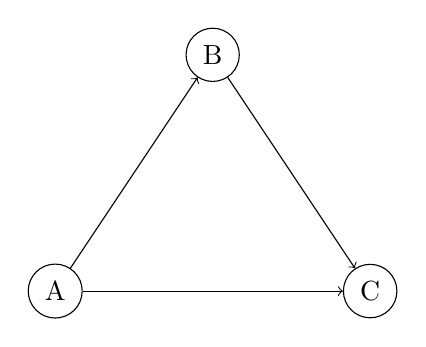
\begin{tikzpicture}
  % Nodes
  \node[circle, draw] (A) at (0,0) {A};
  \node[circle, draw] (B) at (2,3) {B};
  \node[circle, draw] (C) at (4,0) {C};
  
  % Edges
  \draw[->] (A) -- (B);
  \draw[->] (B) -- (C);
  \draw[->] (A) -- (C);
\end{tikzpicture}

\end{frame}

\begin{frame}
\frametitle{Ascension in General}

$\mathscr{F}T$
\end{frame}

\section{Debugging System}
\begin{frame}
test frame for section one
\end{frame}

\section{Regular Feautures}
\begin{frame}
\frametitle{Regular Features}
This section we will discuss the regular features of Husky.

\begin{itemize}
	\item functions
	\item methods
	\item values
	\item type definitions
\end{itemize}
\end{frame}

\begin{frame}
\frametitle{Regular Features: Type Definition}

One can define
\begin{itemize}
	\item regular struct/structure
	\item tuple struct/structure
	\item enum/inductive
	\item 
\end{itemize}
\end{frame}

\begin{frame}
\frametitle{Regular Features: Borrow Checking}
\end{frame}

\begin{frame}
\frametitle{Regular Features: Decorators}
must\_use, no\_discard

\end{frame}

\begin{frame}
\frametitle{Regular Features: Monad through Effect and Unveil}
\end{frame}

\begin{frame}
\frametitle{Regular Features: Incremental Code Analysis}
\end{frame}

\begin{frame}
\frametitle{Regular Features: Incremental Compilation}
\end{frame}

\begin{frame}
\frametitle{Regular Features: Affine Type}
\end{frame}

\begin{frame}
\frametitle{Regular Features: Lifetime and Place}
\end{frame}

\begin{frame}
\frametitle{Regular Features: Generics}
\end{frame}

\begin{frame}
\frametitle{Regular Features: Dependent Types}
\end{frame}

\section{Development Progress}


\end{document}